\documentclass[12pt]{amsart}
\usepackage{marktext} 
%% Remove draft for real article, put twocolumn for two columns
\usepackage{svmacro}
\usepackage[utf8]{inputenc}
\usepackage{lineno}
\usepackage[style=alphabetic, backend=biber]{biblatex}
\addbibresource{bibliography.bib}

%% commentary bubble
\newcommand{\SV}[2][]{\sidenote[colback=green!10]{\textbf{SV\xspace #1:} #2}}

%% Title 
\title{ MATH 102: Homework 5}
\author{Due date: Tues, Nov 14}

%\author{Co-author}
%\address{  }
%\email {  }
%
\date{\today}

\begin{document}

\maketitle

\begin{problem}
    Describe $\R \times \N$ using set notation.
    What is a graphical representation of this set? (For this, make sure you know
    how to insert figures in LaTeX).
\end{problem}


\begin{problem}
    \begin{enumerate}
        \item Is the set $([0,1] \cup [1,2]) \times ([2,3] \cup [3,4])$ the same with 
    $([0,1]\times [2,3])\cup ([1,2]\times [3,4])$?
        \item Let  $A,B,C,D$ be sets. What must be true for the relationship between $(A\cup B) \times (C\cup D)$
    and $(A\times B) \cup (B\times D)$?
        \item Prove your claim in (2).
    \end{enumerate}
\end{problem}

\begin{problem}
    Prove that 
    \begin{enumerate}
        \item $A \times (B\cap C) =  (A\times B) \cap (A \times C)$
        \item $(A\cap B) \times (C\cap D)= (A\times B) \cap (B\times D)$
    \end{enumerate}
\end{problem}


\begin{problem}
    Let $R$ be a relation from $A$ to $B$ and $S$ be a relation from $B$ to $C$.
    We define the composition of relations $S\circ R$ as follows
    \begin{equation*}
        S \circ R = \set{ (a,c) \in A\times C \st \exists b \in B, (a,b) \in R \wedge (b,c) \in S  }\,.
    \end{equation*}

    Consider the following graphs.

    \begin{figure}[ht]
        \begin{center}
            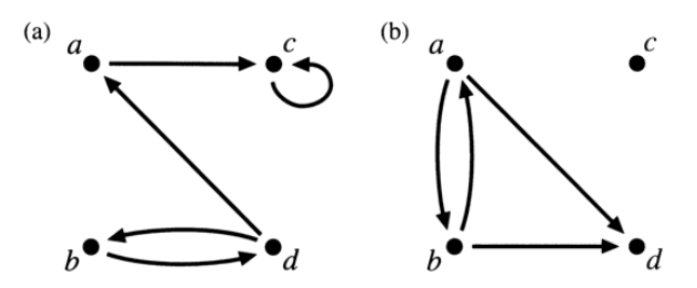
\includegraphics[width=0.95\textwidth]{graph}
        \end{center}
    \end{figure}

    Let $R$ be the relation in (a) and $S$ be the relation in (b).
    \begin{enumerate}
        \item Write, in set notation, $S \circ R$.
        \item Draw $S\circ R$.
    \end{enumerate}
\end{problem}




\printbibliography 
%\bibliography{refs}
%\bibliographystyle{halpha-abbrv}


\end{document}
